\documentclass[a4paper,12pt]{article}
\usepackage[utf8]{inputenc}
\usepackage[spanish]{babel}
\usepackage{graphicx}
\usepackage{float}
\usepackage{url}


%opening
\title{Tarea No. 4. MVC}
\author{Barrera Pérez Carlos Tonatihu \\ Profesor: José Asunción Enríquez Zárate 
\\ Web Application Development \\ Grupo: 3CM9 }

\begin{document}

\maketitle
\newpage
\tableofcontents

\newpage
\section{Introducción}
El modelo vista controlador es una patron de arqutectura de 
software que se usa para implementar interfaces de usuario, por lo 
que es una buena opción en el desarrollo de aplicaciones web.

Separa la lógica de la aplicación en tres partes, promoviendo la 
modularidad, la facilidad de colaboración y la reutilización.\cite{firefox}

\section{Desarrollo}
Se trata de un modelo muy maduro y que ha demostrado su validez a lo largo de 
los años en todo tipo de aplicaciones y sobre multitud de lenguajes y 
plataformas de diseño \cite{uni}.

\begin{figure}[H]
\begin{center}
 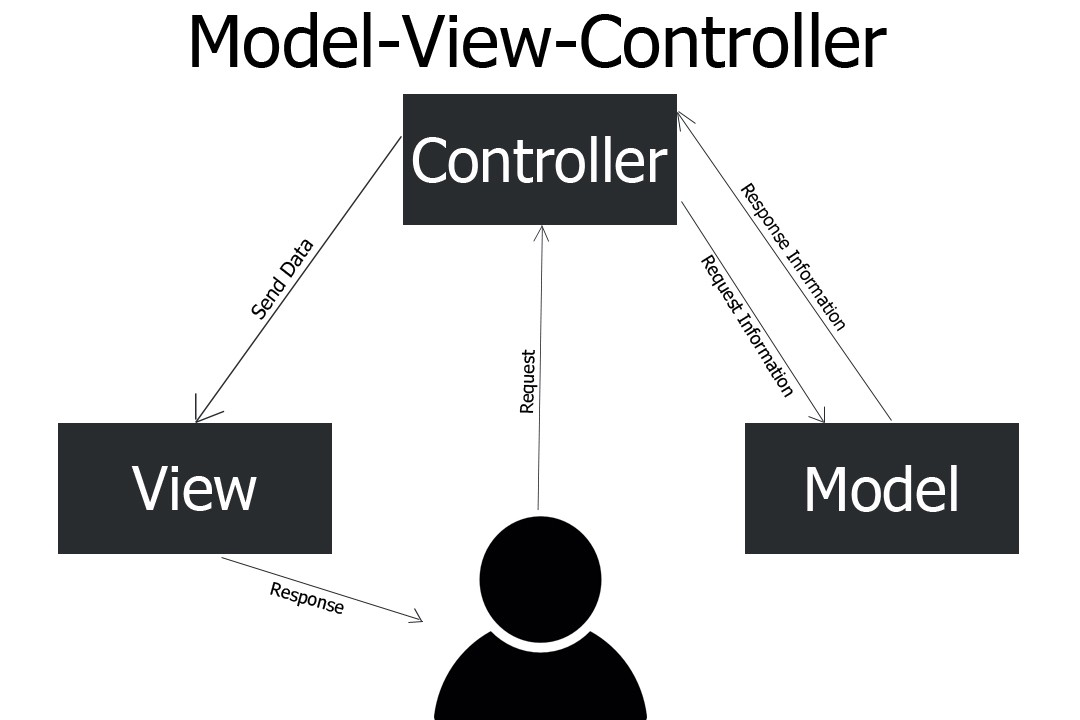
\includegraphics[width=12cm]{modelo.jpg}
 % estructura.png: 800x436 px, 96dpi, 21.16x11.53 cm, bb=0 0 600 327
 \caption{Flujo dentro del MVC}
 \label{fig:control}
\end{center}
\end{figure}

El flujo de control como se muestra en la figura \ref{fig:control} suele ser el 
siguiente:

\begin{enumerate}
  \item El usuario interactúa con la interfaz de usuario de alguna forma (por 
ejemplo, el usuario pulsa un botón, enlace, etc.)
  \item El controlador recibe (por parte de los objetos de la interfaz-vista) 
la notificación de la acción solicitada por el usuario. El controlador gestiona 
el evento que llega, frecuentemente a través de un gestor de eventos (handler) 
o callback.
  \item El controlador accede al modelo, actualizándolo, posiblemente 
modificándolo de forma adecuada a la acción solicitada por el usuario (por 
ejemplo, el controlador actualiza el carro de la compra del usuario). Los 
controladores complejos están a menudo estructurados usando un patrón de comando 
que encapsula las acciones y simplifica su extensión.
  \item El controlador delega a los objetos de la vista la tarea de desplegar 
la interfaz de usuario. La vista obtiene sus datos del modelo para generar la 
interfaz apropiada para el usuario donde se refleja los cambios en el modelo 
(por ejemplo, produce un listado del contenido del carro de la compra). El 
modelo no debe tener conocimiento directo sobre la vista. Sin embargo, se podría 
utilizar el patrón Observador para proveer cierta indirección entre el modelo y 
la vista, permitiendo al modelo notificar a los interesados de cualquier 
cambio. Un objeto vista puede registrarse con el modelo y esperar a los 
cambios, pero aun así el modelo en sí mismo sigue sin saber nada de la vista. 
El controlador no pasa objetos de dominio (el modelo) a la vista aunque puede 
dar la orden a la vista para que se actualice. Nota: En algunas implementaciones 
la vista no tiene acceso directo al modelo, dejando que el controlador envíe 
los datos del modelo a la vista.
  \item La interfaz de usuario espera nuevas interacciones del usuario, 
comenzando el ciclo nuevamente.

\end{enumerate}

\subsection{Modelo}
El Modelo que contiene una representación de los datos que maneja el sistema, su 
lógica de negocio, y sus mecanismos de persistencia.
El modelo es responsable de:

\begin{itemize}
  \item Acceder a la capa de almacenamiento de datos. Lo ideal es que el modelo 
sea independiente del sistema de almacenamiento.
  \item Define las reglas de negocio (la funcionalidad del sistema). Un ejemplo 
de regla puede ser: "Si la mercancía pedida no está en el almacén, consultar el 
tiempo de entrega estándar del proveedor".
  \item Lleva un registro de las vistas y controladores del sistema.
  \item Si estamos ante un modelo activo, notificará a las vistas los cambios 
que en los datos pueda producir un agente externo (por ejemplo, un fichero por 
lotes  que actualiza los datos, un temporizador que desencadena una inserción, 
etc.).
\end{itemize}

\subsection{Vista}
La Vista, o interfaz de usuario, que compone la información que se envía al 
cliente y los mecanismos interacción con éste.
La vista es responsable de:

\begin{itemize}
  \item Recibir datos del modelo y los muestra al usuario.
  \item Tienen un registro de su controlador asociado (normalmente porque 
además lo instancia).
  \item Pueden dar el servicio de "Actualización()", para que sea invocado por 
el controlador o por el modelo (cuando es un modelo activo que informa de los 
cambios en los datos producidos por otros agentes).
\end{itemize}

\subsection{Controlador}
El Controlador, que actúa como intermediario entre el Modelo y la Vista, 
gestionando el flujo de información entre ellos y las transformaciones para 
adaptar los datos a las necesidades de cada uno.
El controlador es responsable de:
\begin{itemize}
  \item Recibe los eventos de entrada (un clic, un cambio en un campo de texto, 
etc.).
  \item Contiene reglas de gestión de eventos, del tipo "Si Evento Z, entonces 
Acción W". Estas acciones pueden suponer peticiones al modelo o a las vistas.
\end{itemize}

\section{Conclusión}
Es un hecho que el Modelo Vista Controlador se ha vuelto todo un estándar en la 
industria, por lo cual se debe de entender el como se utiliza y con ello hacer 
un buen uso de este y acoplarlo de acuerdo a las necesidades que se presenten 
en el desarrollo del proyecto.

\bibliographystyle{ieeetr}
\bibliography{referencias}


\end{document}
